\chapter{2014}
\section*{一、选择题(本大题共 20 小题,每小题 2 分,共 40 分)}

1. 下面程序段的时间复杂度是 (  )。
\begin{lstlisting}[language=C, basicstyle=\ttfamily]
for i=0;i<m;i++)
    A[i]=0;
for(i=0;i<m;i++)
    for (j=1;j<n;j++)
        A[i]+=5;
\end{lstlisting}

A \(\mathrm{O}\left( {\mathrm{m} + \mathrm{n}}\right)\) B \(\mathrm{O}\left( {\mathrm{m} + \mathrm{n} + 1}\right)\) C O(n) D \(\mathrm{O}\left( {{\mathrm{m}}^{ * }\mathrm{n}}\right)\)

2. 计算机算法指的是 (  ), 它必须具备输入、输出和可行性、确定性和有穷性等 5 个特性。。

A 计算方法 B 排序方法

C 解决问题的有限指令序列 D 调度方法

3. 若某栈的输入序列为 1,2,3,..., n,输出序列的第 2 个元素为 n,则第 3 个输出元素为 (  )。

A 1 或 2 B 1 或 \(\mathrm{n} - 1\) C \(\mathrm{n} - 1\) 或 \(\mathrm{n} - 2\) D \(\mathrm{n} - 1\)

4. 线性表的链式存储结构与顺序(连续)存储结构相比优点是(  )。

A. 便于插入和删除 B. 便于随机存取

C. 所有的操作/运算的算法简单 D. 便于查找

5. 设循环队列中数组的下标范围是 \(0..\mathrm{n} - 1\) ,其头指针 front 指向队首元素, rear 指向队尾元素,则队列的长度为(  )。

A rear-front B rear-front + 1

C (rear-front +1) \% (n+1)

D (rear-front \(+ \mathrm{n} + 1\) ) \%n

6. 如果某应用在线性表中最常用的操作是在最后一个元素之后插入一个元素和删除第一个元素, 则采用 (  ) 存储方式最节省运算时间。

A. 仅有头指针的单链表 B. 仅有头指针的单循环链表

C. 双链表 D. 仅有尾指针的单循环链表

7. 在长度为 \(\mathrm{n}\) 且带头结点的链式存储实现的线性表的第 \(\mathrm{i}\left( {0 \leq  \mathrm{i} \leq  \mathrm{n}}\right)\) 个位置插入一个元素, 需要查找运算( )次。

A. 1 B. n-i C. i D. n-2

8. 在长度为 \(\mathrm{n}\) 顺序实现的线性表的第 \(\mathrm{i}\left( {1 \leq  \mathrm{i} \leq  \mathrm{n}}\right)\) 个位置之前插入一个元素,需要后移 \(\left( \right)\) 个元素。

A. i B. n-i+1 C. n D. 1

9. 数组 A 中,每个元素 A 的长度为 4 个字节,行下标 i 从 1 到 8 ,列下标 j 从 1 到 10 , 从首地址 \(\mathrm{S}\) 开始连续存放在存储器内,该数组按行优先存放时,元素 \(\mathrm{A}\left\lbrack  5\right\rbrack  \left\lbrack  6\right\rbrack\) 的起始地址为(  )。

A. S+160 B. S+180 C. S+220 D. S+140

10. 设高度为 \(\mathrm{h}\) 的二叉树上只有度为 0 和度为 2 的结点,则此类二叉树中所包含的结点数至少为(  )。

A. \(2\mathrm{\;h} - 1\) B. \(2\mathrm{\;h}\) C. \(2\mathrm{\;h} + 1\) D.h+1

11. 已知完全二叉树有 10 个结点, 则整棵二叉树有 (  ) 个度为 1 的结点

A. 2 B. 1 C. 0 D. 不确定

12. 在所有排序方法中,关键字比较的次数与记录的初始排列次序无关的是(  ).

A. 直接插入排序 B. 希尔(Shell)排序

C. 简单选择排序 D 冒泡排序

13. 在常用的哈希表处理冲突的方法中,(  )方法容易产生 “二次聚集”,导致哈希表性能变差。

A. 开放定址法一线性探测 B. 再哈希法 C. 链地址法

E. 开放定址法一二次探测

14. 对包含 \(n\) 个元素的散列表进行查找,平均查找长度 (  )

A. 为 \(O\left( {{\log }_{2}n}\right)\) B. 为 \(O\left( n\right)\) C. 不直接依赖于 \(n\) D. \(O\left( {n{\log }_{2}n}\right)\)

15. 对一棵二叉排序 (升序、查找) 树的根结点而言, 左子树中所有结点的关键字都 (  ) 右子树中所有结点的关键字。

A. 不等于 B. 不大于 C. 等于 D. 大于

16. 在对 \(\mathrm{n}\) 个关键字进行简单选择排序的过程中,每一趟都要从无序区选出最小关键字元素,则在进行第 \(\mathrm{i}\) 趟排序之前,无序区中关键字元素的个数为 (  )

A. i B. \(\mathrm{i} + 1\) C. n-i D. n-i+1

17. 下面的关键码序列中哪一个是堆( ？ )。

A.18,72,35,23,94,53 B.18,31,23,94,53,72

C.18,53,23,94,40,72 D.94,55,18,72,16,23

18. 设连通图 G 采用邻接表存储,则深度优先遍历算法的时间复杂度是(  )。

A.O(n) B.O(n+e) C. \(O\left( {n}^{2}\right)\) D.O(n*e)

注: 所有答案必须写在答题纸上, 试卷上作答无效 !

19. 已给右图,(  )是该图的拓扑排序？

A.1,2,3,4,5

\begin{center}
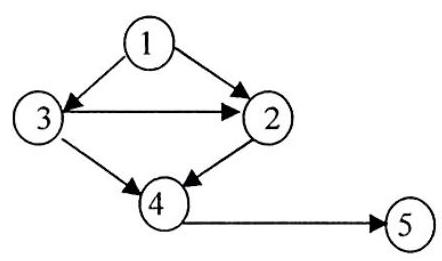
\includegraphics[width=0.3\textwidth]{images/2014/choice_19.jpg}
\end{center}
\hspace*{3em} 

B.1,2,4,3,5

C.1,3,2,4,5

D.1,2,3,5,4

20. 图的邻接矩阵表示法适用于表示 (  )

A. 稠密图 B. 有向图 C. 无向图 D. 稀疏图

\section*{二、填空题(本大题共 17 小题,每小题 2 分,共 34 分)}

1. 设一循环队列 \(\mathrm{Q}\) 中, rear 指针指向队尾元素的下一个位置, front 指针指向队首元素, 则判断队列中元素为空的条件是\_\_\_\_\_\_\_\_。

2. 设栈 \(\mathrm{S}\) 和队列 \(\mathrm{Q}\) 的初始状态皆为空,元素 \(\mathrm{a}1,\mathrm{a}2,\mathrm{a}3,\mathrm{a}4,\mathrm{a}5,\mathrm{a}6\) 和 \(\mathrm{a}7\) 依次通过一个栈,一个元素出栈后即进入队列 \(\mathrm{Q}\) ,若 7 个元素出队列的顺序是 \(\mathrm{a}3,\mathrm{\;a}5,\mathrm{\;a}4,\mathrm{\;a}7,\mathrm{\;a}6\) , a2, a1 则栈 S 至少应该容纳\_\_\_\_\_\_\_\_个元素。

3. 广义表 L \(= \left( {{\left( a\right) }_{3}\left( {b,c}\right) ,\left( d\right) }\right) ,L\) 的长度是\_\_\_\_\_\_\_\_。

4. 二叉树中第 5 层上(根在第 1 层)的结点个数最多为\_\_\_\_\_\_\_\_。

5. 某算法中的语句频度之和为 \(T\left( n\right)  = 3{n}^{2} + {2n} + 7\) ,则其时间复杂度为\_\_\_\_\_\_\_\_。

6. 某表达式语法树(二叉树)按后序遍历的结果为 abc-d+*h-,令 a=2, b=6, c=4, d=5, h=8,则该表达式的值等于\_\_\_\_\_\_\_\_。

7. 采用特殊字符作为结尾的顺序存储方式存储,若两个串的长度分别为 \(\mathrm{m}\) 和 \(\mathrm{n}\) ,则两个串相等与否的比较运算的时间复杂度为\_\_\_\_\_\_\_\_。

8. n 阶矩阵中三角矩阵使用压缩存储方式时需要\_\_\_\_\_\_\_\_个数据元素空间来存储。

9. 一棵含有 20 个结点的二叉树的高度至少为\_\_\_\_\_\_\_\_(空树高度为 0)。

10. 已知某二叉树的先序序列 ABCFDG, 中序序列 CBDFAG, 那么它的后序遍历序列是\_\_\_\_\_\_\_\_。

11. 含 \(\mathrm{n}\) 个顶点的无向连通图中至少含有\_\_\_\_\_\_\_\_条边。

12. 采用特殊字符作为结尾的顺序存储方式存储, 则串 “GLuckyUProgram” 至少\_\_\_\_\_需要个字符的存储空间。

13. 请指出在顺序表 \(\{ 3\text{ 、 }6\text{ 、 }8\text{ 、 }{10}\text{ 、 }{14}\text{ 、 }{15}\text{ 、 }{18}\text{ 、 }{36}\text{ 、 }{44}\text{ 、 }{62}\}\) 中,用二分法/折半法查找关键码 10 需做\_\_\_\_\_\_\_\_次关键码比较。

14. 高度为 5 的 AVL 树(平衡二叉树)至少有\_\_\_\_\_\_\_\_个结点。(空树高度为 0)

15. 应用 Dijkstra's 算法(单源最短路径)求下图顶点 \(\mathrm{A}\) 到顶点 \(\mathrm{D}\) 的最短路径,第 1 步、第 2 ”步求出的是顶点 \(\mathrm{A}\) 到顶点\_\_\_\_\_\_\_\_, \({\mathrm{A}}^{\prime }\) 到顶点\_\_\_\_\_\_\_\_的最短路径。

\begin{center}
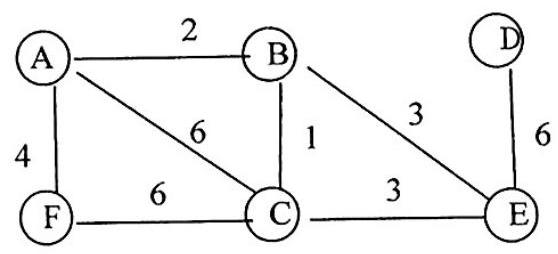
\includegraphics[width=0.4\textwidth]{images/2014/blank_15.jpg}
\end{center}
\hspace*{3em} 

16. 对于键值序列 \(\{ {16},{85},{28},{58},{17},5,{18},{25},{81},{32},{98}\}\) ,建里初始堆,必须从键值为\_\_\_\_\_\_\_\_ 的结点开始对前面的每个结点进行一次堆调整。

17. 排序过程中,对尚未确定最终位置的所有数据元素进行一遍处理称为一趟排序,下列五种排序方法中,每一趟排序结束时都至少能够确定一个元素最终位置的方法有\_\_\_\_\_\_\_\_

I. 简单选择排序 (Shell) 排序 III. 快速排序

IV. 维排序 V. 两路归并排序

\section*{三、问答题(本大题共 8 小题,每小题 7 分,共 56 分)}

1. 在顺序表中插入一个结点需平均移动多少个结点 分析此操作的时间复杂度。

2. 设下图为某树的二叉树表示, 请画出该树。

\begin{center}
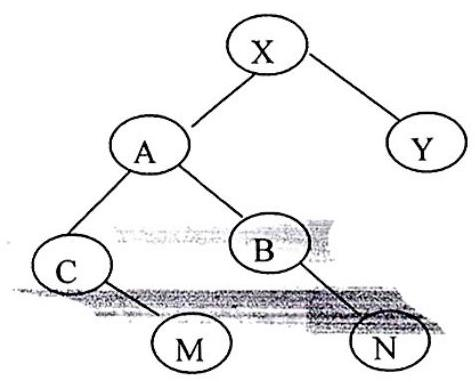
\includegraphics[width=0.4\textwidth]{images/2014/ask_2.jpg}
\end{center}
\hspace*{3em} 
\vspace{5em}

\newpage
3. 已知关键字序列为45,32,22,37,70,42,依次将各元素插入到一棵初始为空的二叉排序树, 画出对应的二叉排序树。
\vspace{10em}

4. 简要说明快速排序的排序思想, 并给出算法时间复杂度。根据所给序列 (50,25,35,80,90,15,99,68),设选第一个元素为支点/参考值 (pivot), 采用双向交替向中间扫描的方式, 写出快速排序的第一趟排序的结果。
\vspace{10em}

\newpage
5. 下图有六个顶点 A、B、C、D、E、F,其连接关系及相应权值如图所示。 给出邻接矩阵表示结果, 然后从顶点 \(\mathrm{A}\) 开始对图进行广度优先遍历, 写出遍历结果。

\begin{center}
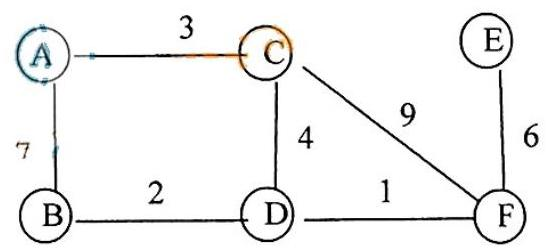
\includegraphics[width=0.4\textwidth]{images/2014/ask_5.jpg}
\end{center}
\hspace*{3em} 
\vspace{12em}

6. 使用 Kruskal 算法求第 5 题所给图 (上图) 的最小生成树, 必须给出树的生成过程。
\vspace{15em}

\newpage
7. 已给输入关键字序列 \(\{ {23},{12},{17},{60},{30},{36},{40},{42}\}\) ,哈希函数为 \(\mathrm{H}\) (key) = key \%9, 哈希表的地址空间为 0, 1, ..., 8, 开始时哈希表为空, 用线性探测法解决冲突, 请依次画出插入键值后的 Hash (哈希) 表, 出现冲突时单独标示清楚。
\vspace{12em}

8. 假设用于通信的电文由字符集 \(\{ X,Y,C,D,F\}\) 中的字母构成,这 5 个字母在电文中出现的频率依次为 \(\{ {35},{20},{10},{13},{22}\}\) 。请画出对应的编码哈夫曼树 (Huffman)。
\vspace{15em}

\section*{四、算法设计、分析题(本大题共 2 小题, 每小题 10 分, 共 20 分)}

1. 现有二叉平衡树(或为空树,或者根结点的左右子树高度差最大为 1 且左、 右子树为二叉平衡树), 试设计一算法判断该二叉树是否为二叉平衡树。

1)先给出设计思想；

2)再描述具体算法, 必要时请给予注释说明。
\vspace{15em}
\vspace{15em}

2. 现有某比赛活动中某选手的 \(\mathrm{n}\) 个评分结果 (百分制,已知都在 60 以上的整数)已存入顺序表中,并且已按升序排序。为了分析相关规律, 现需分析评分的 k -均值直方图(以当前分数为中位数(位置在中间),计算最邻近的 k 个分数平均值并取为整数, 然后统计分数的频率得到。若当前分左边或右边数据不足时直接忽略, 不计入统计数据), 请设计一尽量快速的算法, 求得打印直方图前的统计结果。

1)先给出设计思想；

2)再描述具体算法, 必要时请给予注释说明。
